\begin{center} 
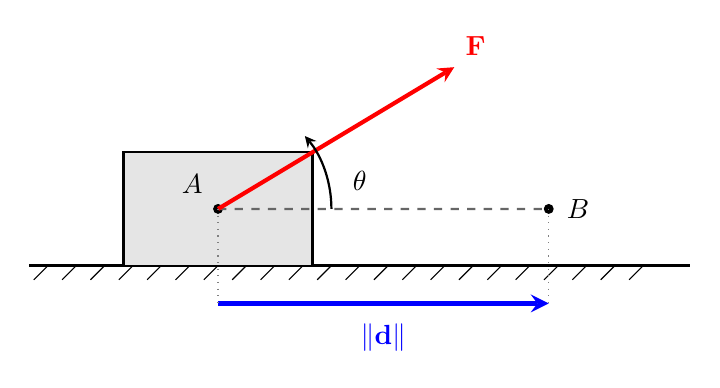
\begin{tikzpicture}[scale=1.2, >=stealth] 

    % 1. Piso / Superficie de apoyo con textura
    \draw[line width=1pt] (-1,0) -- (6,0); 
    \foreach \x in {-0.8,-0.5,...,5.8} {
        \draw (\x,0) -- (\x-0.15,-0.15); 
    }

    % 2. Bloque / Objeto en gris
    \draw[thick, fill=gray!20] (0,0) rectangle (2,1.2); 
    
    % Centro de masa (Punto A: Posición inicial del objeto)
    \coordinate (CM) at (1,0.6); 
    \fill[black] (CM) circle (1.5pt) node[above left=2pt] {$A$}; 

    % 3. Línea auxiliar horizontal (Dirección del movimiento)
    \draw[dashed, black!60, thick] (CM) -- (4.5,0.6); 
    
    % Punto B: Posición final del centro de masa del objeto tras el desplazamiento
    \fill[black] (4.5,0.6) circle (1.5pt) node[right=3pt] {$B$};

    % 4. Vector Fuerza F saliendo de A
    \draw[->, line width=1.5pt, red] (CM) -- (3.5,2.1) node[above right] {$\mathbf{F}$}; 

    % 5. Ángulo theta entre la fuerza y la dirección del movimiento
    \draw[thick, black, ->] (2.2,0.6) arc (0:40:1.2); 
    \node at (2.5,0.9) {$\theta$}; 

    % 6. Vector Desplazamiento posicionado en el suelo (Une las proyecciones de A y B)
    \draw[->, line width=1.8pt, blue] (1, -0.4) -- (4.5, -0.4) node[midway, below=3pt] {$\|\mathbf{d}\|$}; 
    
    % Líneas de proyección tenues que nacen en los puntos A y B hacia el suelo
    \draw[dotted, black!50] (1,0.6) -- (1,-0.4);
    \draw[dotted, black!50] (4.5,0.6) -- (4.5,-0.4);

\end{tikzpicture} 
\end{center}